\section{Component Interfaces}
In these diagrams are shown the main methods offered by the different interfaces of the components to the users of our application.

\begin{itemize}
    \item  The interface \underline{UserMobileServices} provides all the methods that users will call to manage their requests, data visualization, emergency services and services related to run enrollment and run organization.
    \item The interface \underline{ThirdPartyWebServices} extends the interfaces of the Third Party Web Services subsystem. These interfaces provide all the methods relative to the request of data to users and group of users and also to the visualization of the already accessible data.
   \end{itemize}

\begin{figure}[H]
    \centering
    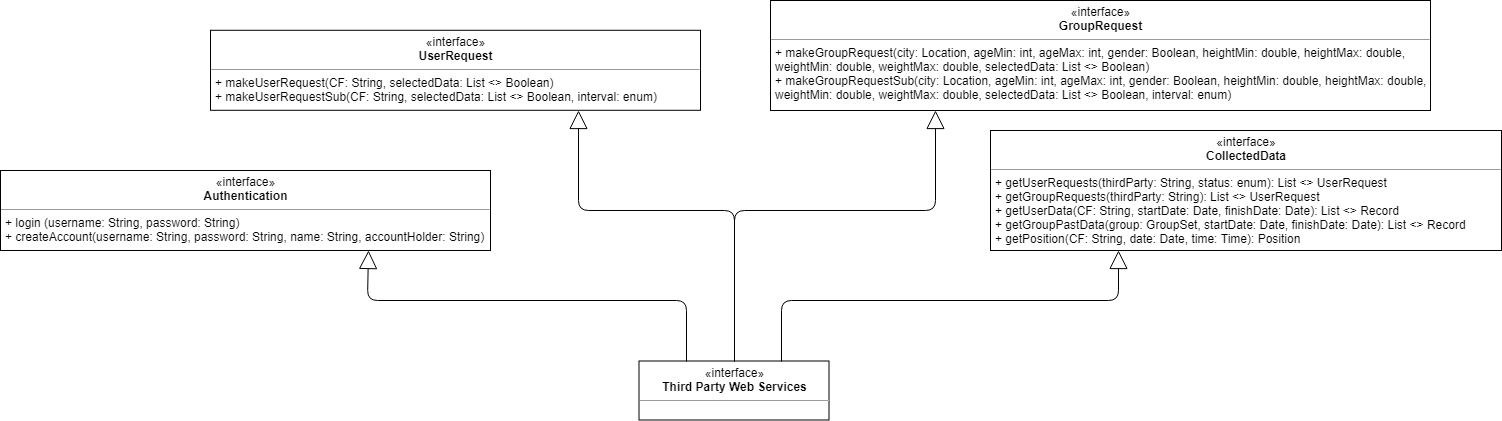
\includegraphics[scale=0.32]{./Pictures/compInterfDiagThirdPDD.png}
   
\end{figure}

\begin{figure}[H]
    \centering
    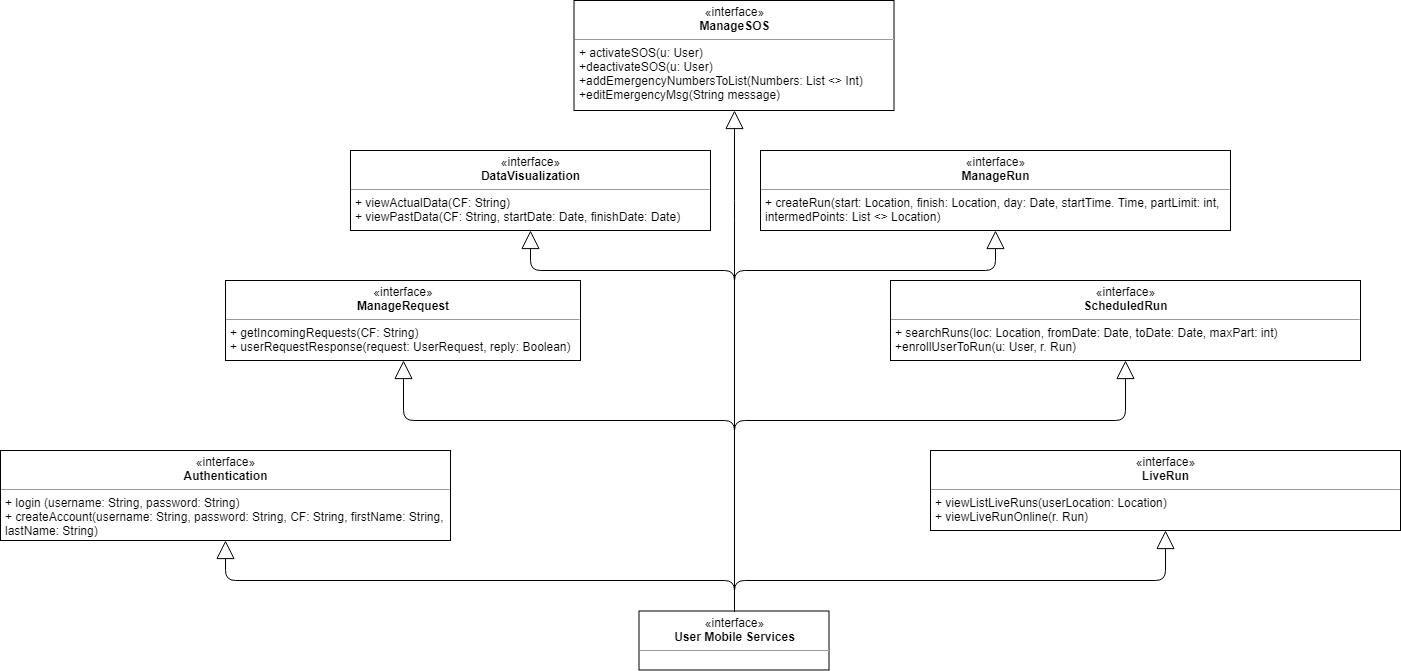
\includegraphics[scale=0.35]{./Pictures/compInterfDiagUserDD.png}
   
\end{figure}